\documentclass{article}

\usepackage{amsmath}
\usepackage{parskip}
\usepackage{tikz}
\renewcommand{\emph}{\textbf}

\begin{document}

\section{Frame 12 -- Functions of Complex Variables}
\textbf{1(a)} 
The function
\[
	f(z) = \frac{1}{z^2 + 1}
\]
is defined everywhere except where $z^2 + 1 = 0$; ie:
\[
	z \neq \pm i
\]

\textbf{1(b)}
The function
\[
	f(z) = \text{Arg}\Big(\frac{1}{z}\Big)
\]
is defined wherever $\frac{1}{z}$ is defined:
\[
	z \neq 0
\]

\textbf{1(c)}
The function
\[
	f(z) = \frac{z}{z + \bar z}
\]
can be written as
\[
	f(x, y) = \frac{x + iy}{(x + iy) + (x - iy)} = \frac{x + iy}{2x} = \frac{1}{2} + i \frac{y}{x}
\]
so the domain is
\[
	\text{Re}(z) \neq 0
\]

\textbf{1(d)}
The function
\[
	f(z) = \frac{1}{1 - |z|^2}
\]
is equivalent to
\[
	f(r, \theta) = \frac{1}{1 - r^2}
\]
so the domain is
\[
	r \neq 1
\]


\textbf{2}
Substituting $z = x + iy$ gives
\begin{align*}
	f(x, y) &= (x + iy)^3 + (x + iy) + 1 \\
	&= x^3 + 3x^2(iy) + 3x(iy)^2 + (iy)^3 + x + iy + 1 \\
	&= (x^3 - 3xy^2 + x + 1) + i(3x^2y - y^3 + y) 
\intertext{so}
	u(x, y) &= x^3 - 3xy^2 + x + 1 \\
	v(x, y) &= 3x^2y - y^3 + y
\end{align*}


\textbf{3}
Using the two expressions
\begin{align*}
	x &= \frac{z + \bar{z}}{2} \\
	y &= \frac{z - \bar{z}}{2i}
\end{align*}
gives
\begin{align*}
	f(z) &= 
	\Big(\frac{z + \bar{z}}{2}\Big)^2 
	- \Big(\frac{z - \bar{z}}{2i}\Big)^2 
	- 2 \frac{z - \bar{z}}{2i} \\
	& \quad + i\Big[2 \frac{z + \bar{z}}{2} \Big(1 - \frac{z - \bar{z}}{2i}\Big) \Big] \\
% 	
	&= \frac{1}{4} (z^2 + 2z\bar{z} + \bar{z}^2 + z^2 - 2z\bar{z} + \bar{z}^2) 
	+ i z - i \bar{z} \\
	& \quad + i \Big[ z + \bar{z} + \frac{iz^2}{2} - \frac{i\bar{z}^2}{2}\Big] \\
%
	&= \frac{1}{2} (z^2 + \bar{z}^2) + 2iz - \frac{iz^2}{2} + \frac{\bar{z}^2}{2} \\
%
	&= \bar{z}^2 + 2iz
\end{align*}


\textbf{4}
Using
\[
	z = re^{i\theta}
\]
the function can be written as
\begin{align*}
	f(z) &= re^{i\theta} + \frac{1}{re^{i\theta}} \\
	&= re^{i\theta} + \frac{1}{r} e^{-i\theta} \\
	&= (r + \frac{1}{r}) \cos \theta + i(r - \frac{1}{r}) \sin \theta
\end{align*}


\clearpage
\section{Frame 14 -- Mappings by the Exponential Function}
\textbf{1}
We saw earlier that the hyperbolas
\[
	x^2 - y^2 = c_1
\]
map onto the horizontal lines $u = c_1$ and the hyperbolas
\[
	2xy = c_2
\]
map onto the vertical lines $v = c_2$. Thus, a domain on the z-plane that maps onto $1 \le u \le 2$ and $1 \le v \le 2$ is
\[
	1 \le x^2 - y^2 \le 2	\quad	1 \le 2xy \le 2
\]
A sketch of this region is:
\begin{center}
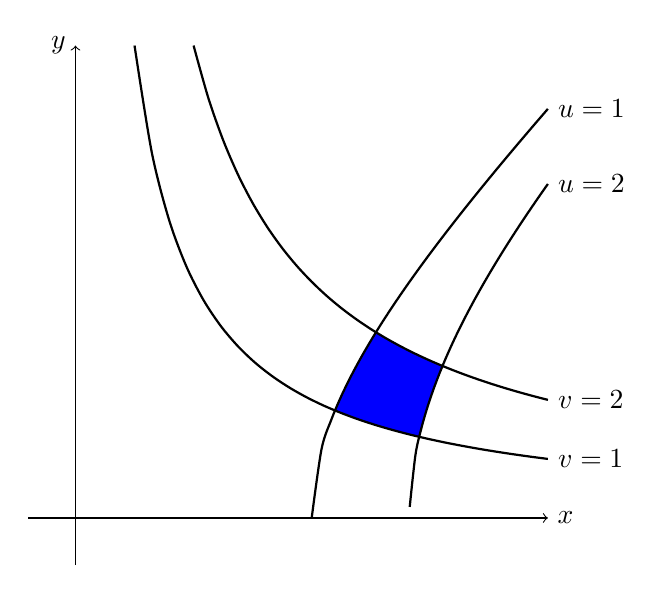
\begin{tikzpicture}[scale=3]
	\draw [->] (-0.2,0) to (2,0) node[right]{$x$};
	\draw [->] (0,-0.2) to (0,2) node[left] {$y$};
	
	\fill [fill=blue]
		plot [domain=1.272:1.554] (\x, {2 / (2*\x)}) --
		plot [domain=1.554:1.455] (\x, {sqrt(\x*\x - 2)}) --
		plot [domain=1.455:1.099] (\x, {1 / (2*\x)}) --
		plot [domain=1.099:1.272] (\x, {sqrt(\x*\x - 1)});
	\draw [thick, domain=0.25:2]  plot [smooth] (\x, {1 / (2*\x)}) node[right]{$v = 1$};
	\draw [thick, domain= 0.5:2]  plot [smooth] (\x, {2 / (2*\x)}) node[right]{$v = 2$};
	\draw [thick, domain=1:2]     plot [smooth] (\x, {sqrt(\x*\x - 1}) node[right]{$u = 1$};
	\draw [thick, domain=1.415:2] plot [smooth] (\x, {sqrt(\x*\x - 2}) node[right]{$u = 2$};
\end{tikzpicture}
\end{center}


\textbf{2}
The first hyperbola can be written as
\[
	y^2 - x^2 = |c_1|
\]
Then, substitution into the $v$ equation gives
\[
	u = c_1, \quad	v = \begin{cases}
		 2x \sqrt{x^2 + |c_1|},	& y > 0 \\
		-2x \sqrt{x^2 + |c_1|},	& y < 0 \\
	\end{cases}
\]
This maps out the entire $v$ line as $x$ moves right (on the top branch) or left (on the bottom branch).

The second hyperbola can be written as
\[
	2xy = -|c_2|
\]
and substituting this into the $u$ equation gives
\[
	u = x^2 - \frac{c_2^2}{4x^2}, 	\quad 	v = c_2 
\]
This maps out the entire $u$ line: as $x$ gets large in magnitude, so too does $u$. A sketch of these mappings is:
\begin{center}
\begin{tikzpicture}[scale=1]
	\draw [->] (-3,0) -- (3,0) node[right]{$x$};
	\draw [->] (0,-3) -- (0,3) node[right]{$y$};
	
	\draw [thick, ->]  plot [domain=-3:3] (\x, { sqrt(\x*\x + 1)});
	\draw [thick, ->]  plot [domain=3:-3] (\x, {-sqrt(\x*\x + 1)});
	\draw [dashed, ->] plot [domain=0.33:3] (\x, {-2 / (2*\x)});
	\draw [dashed, ->] plot [domain=-0.33:-3] (\x, {-2 / (2*\x)});
	
	\draw [->] (4,0) -- (10,0) node[right]{$u$};
	\draw [->] (7,-3) -- (7,3) node[right]{$v$};
	
	\draw [thick, ->] (5,-3) -- (5,3) node[right]{$u = c_1$};
	\draw [dashed, ->] (4,-2) -- (10,-2) node[right]{$v = c_2$};
\end{tikzpicture}
\end{center}


\textbf{3}
The image of the sector $r \le 1, 0 \le \theta \le \pi/4$ under the mapping $w = z^n$ is
\[
	\rho \le 1,	\quad	0 \le \theta \le n\frac{\pi}{4}
\]
A sketch of these images for $n = 2, 3, 4$ is:
\begin{center}
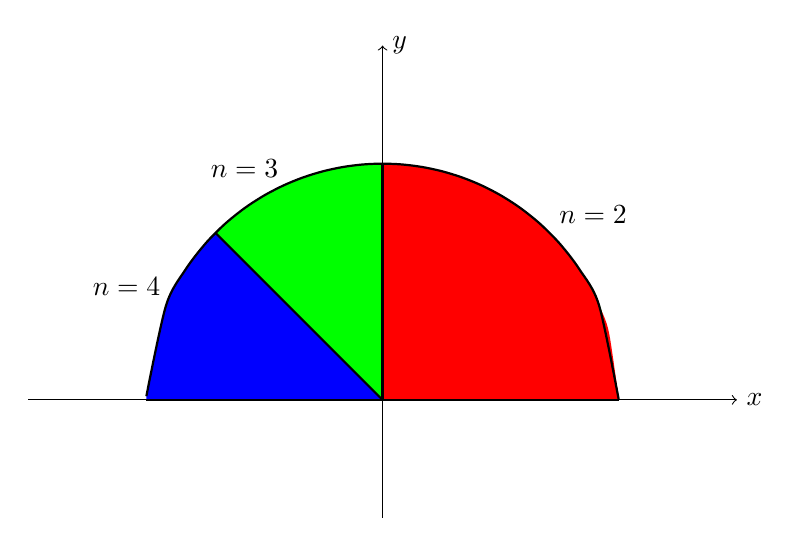
\begin{tikzpicture}[scale=3, smooth]
	\draw [->] (-1.5,0) -- (1.5,0) node[right]{$x$};
	\draw [->] (0,-0.5) -- (0,1.5) node[right]{$y$};
	
	\fill[fill=blue] (1,0) -- plot [domain=1:-1] (\x, {sqrt(1 - \x*\x)}) --
		(-1,0) -- (1,0);
	\fill[fill=green] (1,0) -- plot [domain=1:-0.707] (\x, {sqrt(1 - \x*\x)}) --
		(135:1) -- (0,0) -- (1,0);
	\fill[fill=red] (1,0) -- plot [domain=1:0] (\x, {sqrt(1 - \x*\x)}) --
		(0,0) -- (1,0);
	\draw [thick] (0,0) -- (1,0);
	\draw [thick] (0,0) -- ++ (90:1);
	\draw [thick] (0,0) -- ++ (135:1);
	\draw [thick] (0,0) -- ++ (180:1);
	\draw [thick] plot [domain=1:-1] (\x, {sqrt(1 - \x*\x});
	\node [above right] at (0.707, 0.707){$n = 2$};
	\node [above left] at  (-0.4, 0.9)   {$n = 3$};
	\node [above left] at  (-0.9, 0.4)   {$n = 4$};
\end{tikzpicture}
\end{center}


\textbf{4}
If $z$ follows the straight line $ay = x$, then the mapping $w = e^z$ is
\begin{align*}
	w &= e^{x + iy} \\
	&= e^{ay}e^{iy} \\
	&= e^{a\phi} e^{i\phi} \\
	&= \rho e^{i\phi}
\end{align*}
where $ \rho = a\phi$.


\textbf{5}
The rectangular region $a \le x \le b$, $c \le y \le d$ is made up of the horizontal line segments
\[
	x = t,	\quad	y = c_1
\]
where $t$ is a parameter running from $a$ to $b$ and $c_1$ is a constant in the range $[c, d]$. These horizontal lines have the images
\[
	\rho = e^t,	\quad	\phi = c_1
\]
Since $t$ starts at $a$ and ends at $b$, these images have a radius in the range $[e^a, e^b]$. Then, the entire image is the set of these lines, which range from $\phi = c$ to $\phi = d$. Thus, the entire image is
\[
	e^a \le \rho \le e^b,	\quad	c \le \phi \le d
\]


\textbf{6}
Looking at the $z$ plane, the initial set is the infinite strip
\[
	x \le 0, \quad	0 \le y \le \pi
\]
This maps to the image set
\[
	\lim_{a \to -\infty} e^{a} \le \rho \le e^0,	\quad 0 \le \phi \le \pi
\]
or
\[
	0 \le \rho \le 1,	\quad 0 \le \phi \le \pi
\]
This is the upper half of the unit disk, as shown in the figure.


\textbf{7}
In a similar manner to the previous problem, the image of the strip
\[
	x \ge 0, \quad	0 \le y \le \pi
\]
is the upper half-plane with a unit disk cut out:
\[
	\rho \ge 1,	\quad	0 \le \phi \le \pi
\]
A sketch of this region is:
\begin{center}
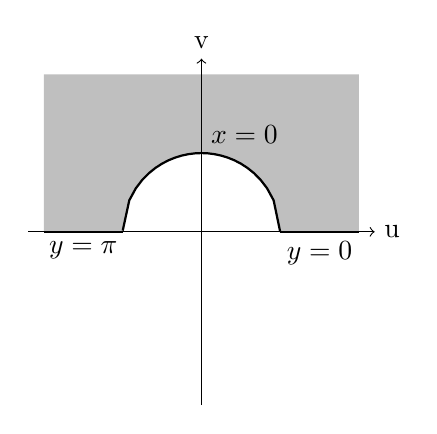
\begin{tikzpicture}	
	\fill [fill=gray!50] (2,0) -- (1,0) -- 
		plot [domain=1:-1] (\x, {sqrt(1 - \x*\x)}) --
		(-1,0) -- (-2,0) -- (-2,2) -- (2,2) -- (2,0);
		
	\draw [->] (-2.2,0) -- (2.2,0) node [right]{u};
	\draw [->] (0,-2.2) -- (0,2.2) node [above]{v};
	
	\draw [thick] (1,0) -- (2,0);
	\node [below] at (1.5,0) {$y = 0$};
	\draw [thick] (-1,0) -- (-2,0);
	\node [below] at (-1.5,0) {$y = \pi$};
	\draw [thick] plot [domain=1:-1] (\x, {sqrt(1 - \x*\x)});
	\node [above right] at (0,1) {$x = 0$};
\end{tikzpicture}
\end{center}


\textbf{8}
Some sample vectors in these two fields are:
\begin{center}
\begin{tikzpicture}
	\draw [->] (-5.5,0)  -- (-0.5,0) node [right]{$x$};
	\draw [->] (-3,-2.5) -- (-3,2.5) node [right]{$y$};
	
	\draw [thick, ->] (-3,0) ++ (1,0) -- ++(90 :0.5);
	\draw [thick, ->] (-3,0) ++ (2,0) -- ++(90 :1);
	\draw [thick, ->] (-3,0) ++ (0,1) -- ++(180:0.5);
	\draw [thick, ->] (-3,0) ++ (0,2) -- ++(180:1);
	\draw [thick, ->] (-3,0) ++ (-1,0) -- ++(270 :0.5);
	\draw [thick, ->] (-3,0) ++ (-2,0) -- ++(270 :1);
	\draw [thick, ->] (-3,0) ++ (0,-1) -- ++(0:0.5);
	\draw [thick, ->] (-3,0) ++ (0,-2) -- ++(0:1);
	
	
	\draw [->] (0.5,0)  -- (5.5,0) node [above right]{$x$};
	\draw [->] (3,-2.5) -- (3,2.5) node [right]{$y$};
	
	\draw [thick, ->] (3,0) ++ (1,0) -- ++(0:0.5);
	\draw [thick, ->] (3,0) ++ (2,0) -- ++(0:1);
	\draw [thick, ->] (3,0) ++ (0,1) -- ++(90:0.5);
	\draw [thick, ->] (3,0) ++ (0,2) -- ++(90:1);
	\draw [thick, ->] (3,0) ++ (-1,0) -- ++(180:0.5);
	\draw [thick, ->] (3,0) ++ (-2,0) -- ++(180:1);
	\draw [thick, ->] (3,0) ++ (0,-1) -- ++(270:0.5);
	\draw [thick, ->] (3,0) ++ (0,-2) -- ++(270:1);
\end{tikzpicture}
\end{center}


\clearpage
\section{Frame 18 -- Limits and Continuity}
\textbf{1(a)}
The left side of the limit is
\[
	|\Re(z) - \Re(z_0)| = |\Re(z - z_0)| < |z - z_0|
\]
so
\[
	|\Re(z) - \Re(z_0)| < \delta \text{ whenever } |z - z_0| < \delta
\]

\textbf{1(b)}
The left side of the limit is
\[
	|\bar{z} - \bar{z_0}| = |\bar{z - z_0}| = |z - z_0|
\]
so the limit holds.

\textbf{1(c)}
The limit expression is
\[
	|\frac{\bar{z}^2}{z}| < \epsilon \text{ whenever } |z| < \delta
\]
For $z \neq 0$, the left side expression is $|z|$, so the limit holds where $\epsilon = \delta$.

\textbf{2}



\end{document}